In this section we describe how we have performed the testing of our system.
We have basically followed the guidelines already defined in our Design document so, if you want additional information, please refer to sections 6.4 and 6.5 of that document.
As regards ApplicationServer subsystem, since in the DD we have described the testing strategy of the entire planned subsystem, we do not have performed the testing of the entire system but only until event EventManager integration (please refer to our design document to see the order of integration).\\
\begin{figure}[H]
	\begin{center}
		\hspace*{-40pt}
		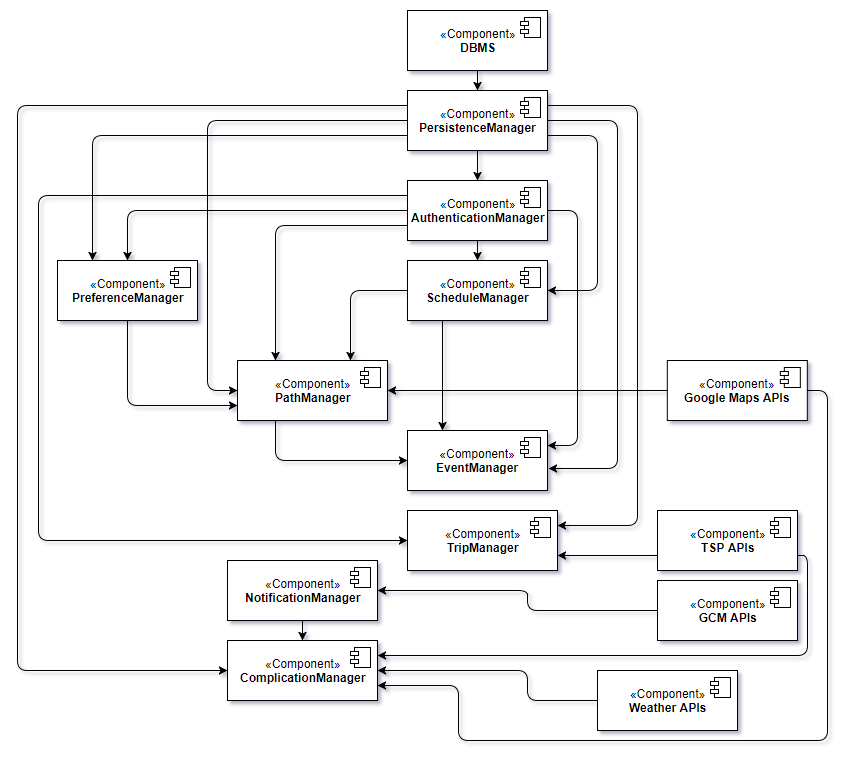
\includegraphics[scale=0.4]{app_server_I&T.png}
	\end{center}
\caption{ ApplicationServer - Actually tested subsystems subsystems}
\end{figure}
As regards Android App subsystem ...\todo{TODO}

\section{Procedure Adopted}
\subsection{Persistence manager (JPA - DBMS interaction): Arquillian}
In order to perform our \textit{PersistenceManager}'s testing we have adopted the following procedure: we have exploited Arquillian features to obtain a testing configuration that allow us to use a testing container of GlassFish that can run and connect to a embedded GlassFish 3.1 instance.
Our \textit{PersistenceManager}'s tests simply  persists a set of sample entities to the database, connected with the GlassFish container, and then retrieve them using JPA Criteria API.
Each test method checks that the sample data retrieved from the database is correct.  Before and after a test is performed, the database is cleaned up, in order to guarantee that each test is run in a clean environment.
This is the outcome of these tests:
\begin{figure}[H]
	\begin{center}
		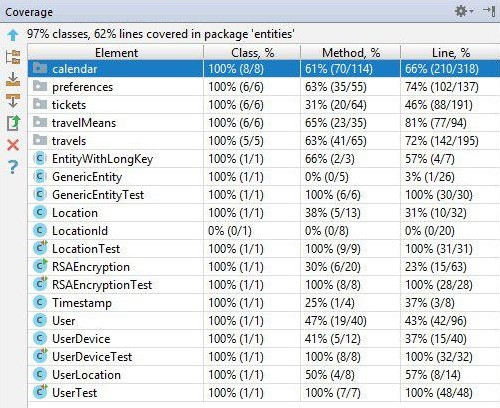
\includegraphics[scale=0.7]{JPA_test_outcome.jpg}
	\end{center}
\caption{ \textit{PersistenceManager} - code coverage}
\end{figure}

\subsection{Enterprise Java Beans: Mockito}
\begin{figure}[H]
	\begin{center}
		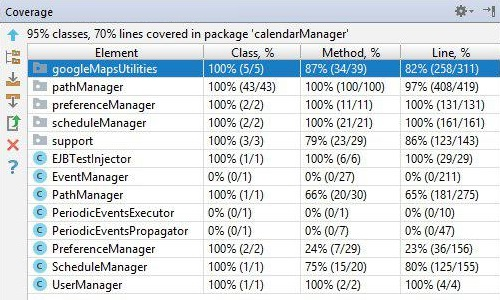
\includegraphics[scale=0.7]{CalendarManager_test_outcome.jpg}
	\end{center}
\caption{ \textit{CalendarManager} - code coverage}
\end{figure}

\subsection{RESTful API: JMeter}


